\section{Implementation Details}
\label{app:impl_details}

% \color{red}
\subsection{Systems Design}

\textbf{Overall Design. } We implement \Sys in a custom inference engine written in PyTorch. Our implementation incorporates PagedAttention \citep{kwon2023efficient}, continuous batching \citep{yu2022orca}, tensor parallelism, BF16 mixed precision, torch compilation, and CUDAGraphs.

The architecture is built around a target model split across 4 devices, and a small draft on a separate device. The two communicate through NCCL once per speculation round, wherein the target sends only the results of the previous round (number of accepted tokens, bonus token sampled), and the draft model uses this to key a lookup into its pre-prepared speculation cache, and immediately returns the tokens and logits corresponding to the pre-prepared speculation on a cache hit, and either random outputs or just-in-time speculation in the case of a cache miss. The key point is that the target model never sees the draft-side speculation cache: it is sent the speculated tokens for its verification outcome immediately after verification. In particular, no KV cache is ever transferred between the devices. 

\textbf{Implementation Details.}
The engine orchestrates from a coordinator process on the main GPU. A scheduler paired with a block manager handles prefill/decode scheduling and page-table bookkeeping. A ModelRunner on each target GPU prepares attention metadata and executes forward passes. In async mode, the draft model runs in a separate process on its own GPU. Target and draft communicate once per iteration via NCCL with fused payloads: the target sends cache keys (sequence ID, accepted-prefix length, recovery token), current sequence lengths, draft block tables for KV addressing, and per-row temperatures; the draft returns a cache-hit bitmap, $K$ speculative tokens per sequence, and $K$-step logits for acceptance.

While the target host maintains page-table bookkeeping for both models, the draft KV cache tensor resides on the draft device. The scheduler ensures the target has sufficient pages for $K+1$ multi-query decoding steps, preempting sequences when lookahead reservations cannot be satisfied. After verification, both page tables are reconciled: completed pages are finalized (hashed for prefix caching), and any pages allocated beyond the accepted suffix are deallocated. This rollback requirement—undoing allocations for rejected tokens that wrote into pre-allocated pages—necessitates a host-side post-processing step after each verification.

\textbf{Design Decisions and Performance Engineering.} During draft speculation, all $F({K+1})$ branches of each sequence are decoded in parallel using a custom sparse attention mask that allows each branch to attend to the verified trunk and its own forking path. We use FlashAttention kernels \citep{shah2024flashattention3} where possible, falling back to FlashInfer \citep{ye2025flashinfer} for multi-query decoding paths requiring custom masks. An example mask is shown in Figure \ref{fig:custom-mask}.

\begin{figure}
\centering
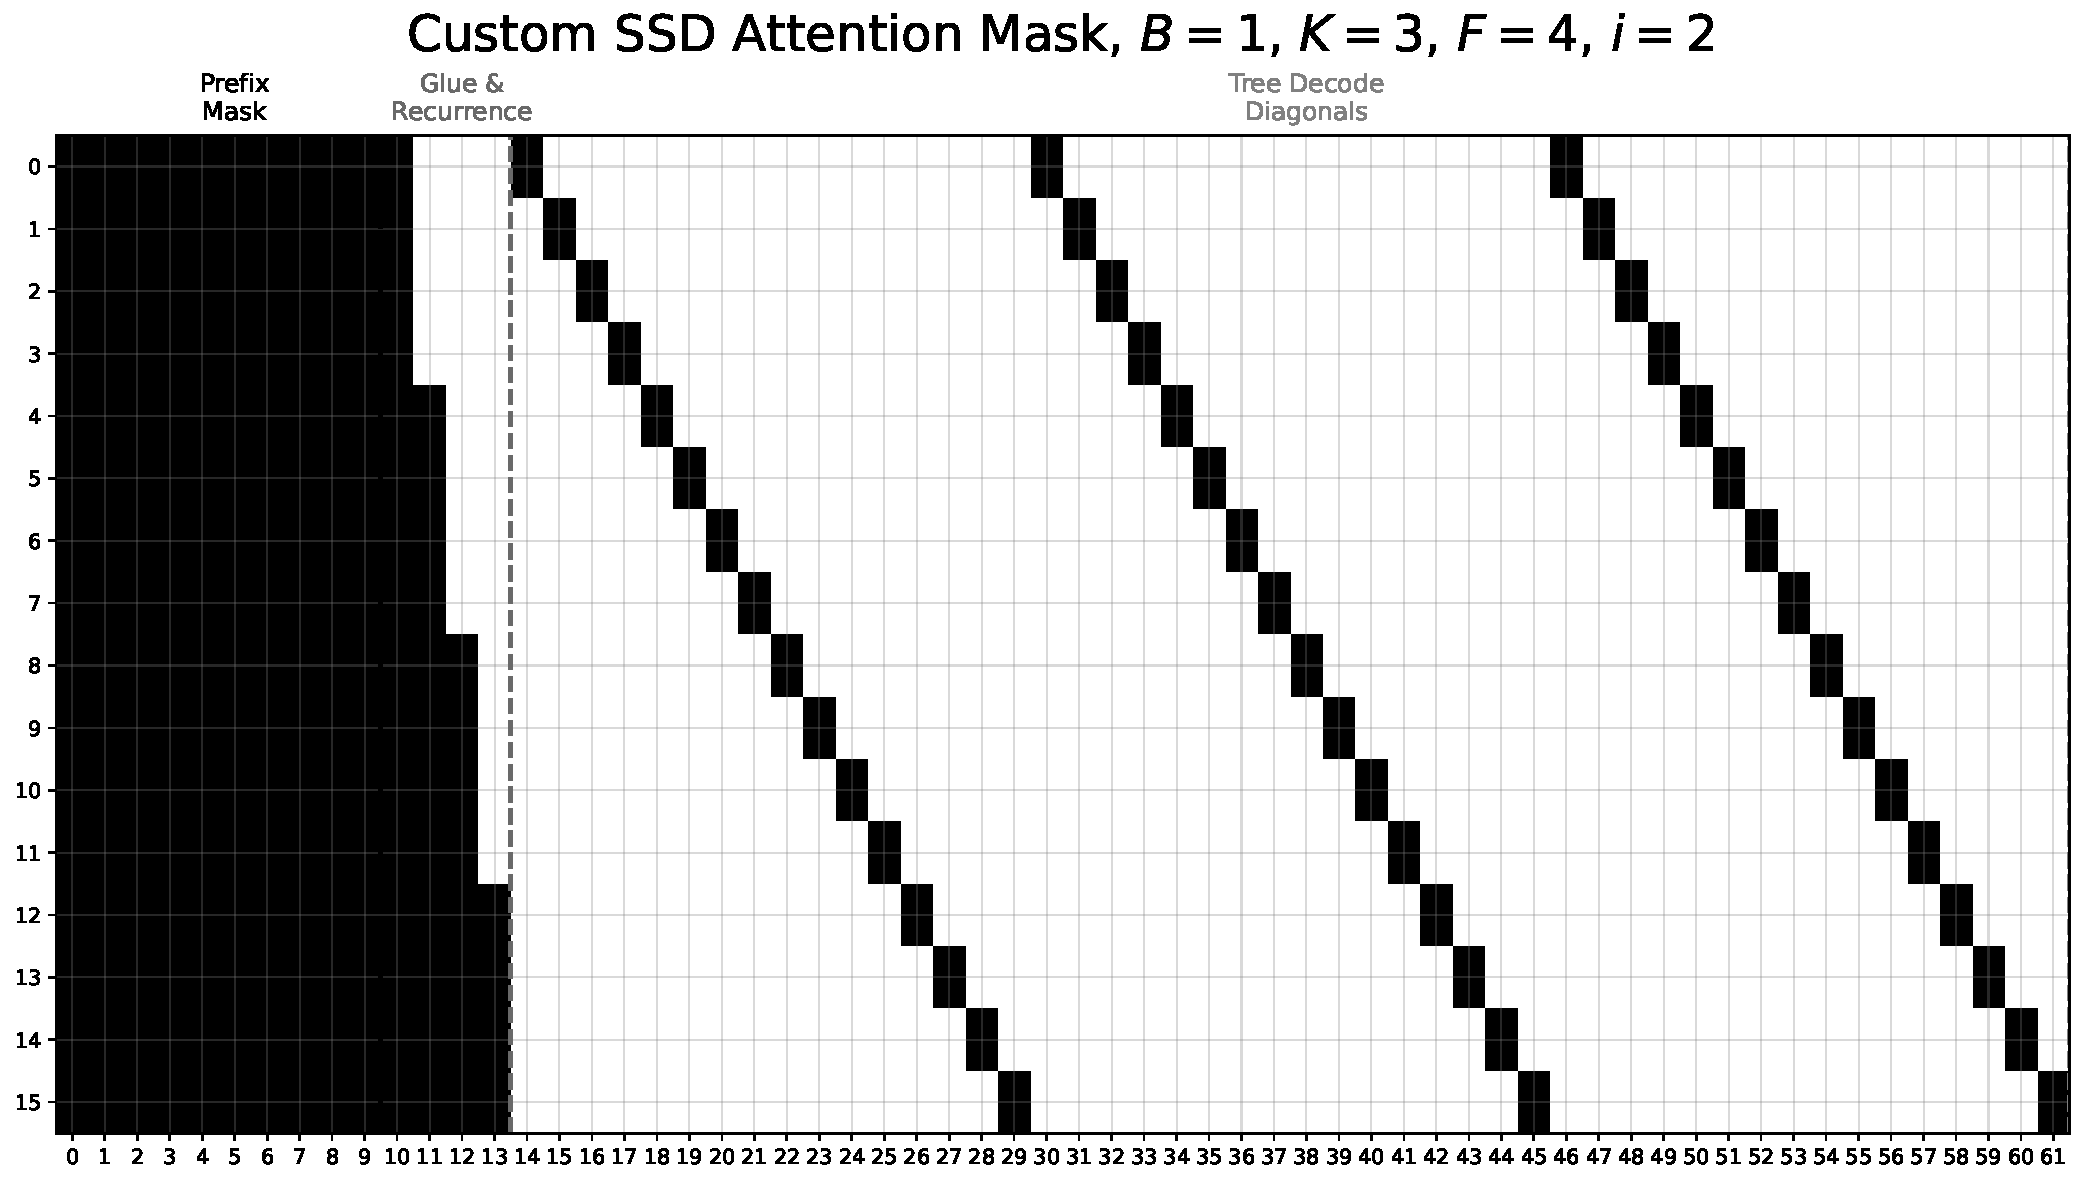
\includegraphics[width=0.65\linewidth]{figures/custom_mask_visualization.pdf}
\caption{
% \color{red}
Custom attention mask for multi-query decoding of all $BF({K+1})$ verification branches in parallel. This mask is for $B=1$, $K=3$, uniform fan-out $F=4$, at depth $i=2$. Black indicates tokens that can be attended to. The left block shows attention to the verified prefix; diagonal bands show each branch attending only within its forking path.}
\label{fig:custom-mask}
\end{figure}

Materializing these masks—which depend on prefix length, $B$, $K$, $F$, and step $i$—is substantial overhead. The sparse, non-coalesced memory access patterns in custom-mask attention kernels dominate our critical path, limiting how many steps we can profitably draft. Thus, most end-to-end speedup comes from hiding draft latency rather than increasing lookahead.
Since accepted branches land in fragmented KV cache locations, we perform an extend (prefill) operation of the previous speculation into KV cache before each round of async decoding. This corresponds to the ``Glue \& Recurrence" column in Figure \ref{fig:custom-mask}, enabling all $F$ forked branches to attend to the same prefix.

\subsection{Experimental Design}

\textbf{Datasets.} We take 128 prompts from each dataset and sample 512 decoding tokens for each. We use vanilla sampling (not top-p or top-k). We measure decoding throughput, excluding prefill. All experiments are done on a single node of NVIDIA H100s, though we only use TP=4 (AR, SD) or 5 (SSD) GPUs at once. 


\textbf{Baselines.} We compare to the two most widely used open-source  
  inference engines: vLLM (v0.16.0) and SGLang (v0.5.9), with
  autoregressive, standalone speculative decoding, and EAGLE-3. All baselines use tensor parallelism across 4$\times$H100 80GB GPUs with greedy decoding, radix caching disabled, and a single concurrent request (batch size 1) unless otherwise specified. For speculative
   decoding, we use Llama-3.2-1B-Instruct as the draft model for
  Llama-3.1-70B-Instruct and Qwen3-0.6B for Qwen3-32B, proposing 5 draft
  tokens per step. We evaluate on 512 prompts drawn equally from
  HumanEval, Alpaca, GSM8K, and UltraFeedback, generating 512 tokens per prompt. Though SSD outperforms tree-based methods like EAGLE-3, it can be combined with these methods---see Appendix~\ref{app:combine}. Our implementation of vanilla speculative decoding has speed comparable to that of vLLM and SGLang confirming it is a strong baseline.

% \color{red}
\subsection{Numerical Results}

\begin{table}[h]
\centering
\small
\setlength{\tabcolsep}{4pt}
\begin{tabular}{lcccccc}
\hline
\textbf{Model} & \textbf{Dataset} & \textbf{AR tok/s} & \textbf{SD tok/s} & \textbf{SSD tok/s} & \textbf{SSD/SD} & \textbf{SSD/AR} \\
\hline
Llama-3.1-Instruct \\ 70B/1B & HumanEval & 54.7 & 176 & 283 & 1.60$\times$ & 5.17$\times$ \\
 & Ultrafeedback & 54.7 & 138 & 215 & 1.55$\times$ & 3.93$\times$ \\
 & Alpaca & 54.7 & 145 & 224 & 1.55$\times$ & 4.10$\times$ \\
 & GSM8k & 54.7 & 188 & 301 & 1.60$\times$ & 5.50$\times$ \\
 & Average & 54.7 & 161.8 & 255.8 & 1.58$\times$ & 4.68$\times$ \\
\hline
Qwen-3 \\ 32B/0.6B & HumanEval & 88.8 & 146 & 222 & 1.52$\times$ & 2.50$\times$ \\
 & Ultrafeedback & 88.8 & 122 & 174 & 1.43$\times$ & 1.96$\times$ \\
 & Alpaca & 88.8 & 127 & 185 & 1.47$\times$ & 2.08$\times$ \\
 & GSM8k & 88.8 & 152 & 234 & 1.54$\times$ & 2.64$\times$ \\
 & Average & 88.8 & 136.8 & 203.8 & 1.49$\times$ & 2.29$\times$ \\
\hline
\end{tabular}
\label{tab:throughput_results}
\end{table}


\section{SSD Overhead}
\label{app:overhead}

Let $B$ be the target batch size, $K$ the speculation lookahead, and $F$ the (uniform) fan out factor for the draft model guessing verification bonus tokens. 

\textbf{Compute.} Let $\hat{c}$ be the compute required for a draft forward pass, normalized by units of target FLOPs. Since the draft decodes $BK(K+1)F$ tokens per round in SSD but $BK$ tokens per round in SD, we incur a factor of $\hat{c}(K+1)F$ more FLOPs on the draft relative to ordinary speculative decoding. Recall this is because each of the $K$ draft steps decodes $B(K+1)F$ tokens in parallel using a custom attention mask. 

In much the same way that SD uses more FLOPs to achieve lower latency (see \citep{leviathan2023}, Section 3.4), SSD applies the same philosophy to use \textit{even more FLOPs} to achieve \textit{even lower latency} than even SD itself. In the SD setting, tokens speculated by the draft that were rejected by the target constitute wasted compute. In the SSD setting (in addition to the above), we have that entire \textit{chains} decoded pre-emptively in parallel for anticipated verification outcomes constitute wasted compute. Thus, SSD introduces new tradeoffs between compute and latency that were not possible before. 

\textbf{Memory.} The draft model must build up a speculation cache as it speculates asynchronously. This has possible verification outcomes as keys and the corresponding tokens/logits as values. Concretely, this means storing a tensor of $BK(K+1)F$ tokens that are decoded, in the form of length-$K$ speculations stored for $B(K+1)F$ possible verification outcomes. For each of these tokens, we also store logits of size $V$, so the speculation cache stores overall $O\left(BFK(K+1)(V+1)\right)$ bits, ending up around hundreds of megabytes in practice. Given this cache is refreshed every speculation round, this ends up small enough to be a non-issue in practice, as the HBM on modern GPUs is much larger. 

\textbf{Communication.} The draft and target model synchronize once per speculation round. The target model sends the outcome of the previous round of speculation (the number of accepted tokens and recovery token for each sequence, $O(B)$ bits of information). The draft sends back the newly speculated tokens (``cache hits") as well as their logits (which the target will need for verification). This is $O(BKV)$ bits of information. All communications are device to device over NCCL via NVLink, which is fast enough that communications are not a bottleneck in practice. 

\color{black}